\chapter{Implementierung}
\label{cha:implementation}

Die Implementierung des Compilers ist in zwei Teile aufgeteilt: Frontend und Backend. Die Kommunikation zwischen den beiden Teilen erfolgt mithilfe eines abstrakten Syntaxbaums (AST), welchen das Frontend erzeugt. Dieses Kapitel geht  auf die Architektur und Implementierung dieser Teile ein.

Die Implementierung erfolgt in Kotlin, was das Einbinden von bereits existierende Bibliotheken des JVM Ökosystems problemlos ermöglicht. Konkret geht es dabei um ANTLR und ObjectWeb ASM, welche wichtige Rollen im Compiler übernehmen. Die Möglichkeit, Summentypen in Form von \textit{sealed} Schnittstellen und Klassen implementieren zu können, erleichert die Abarbeitung des ASTs wesentlich.

\begin{figure}[h]
    \caption{Compiler-Architektur}
    \centering
    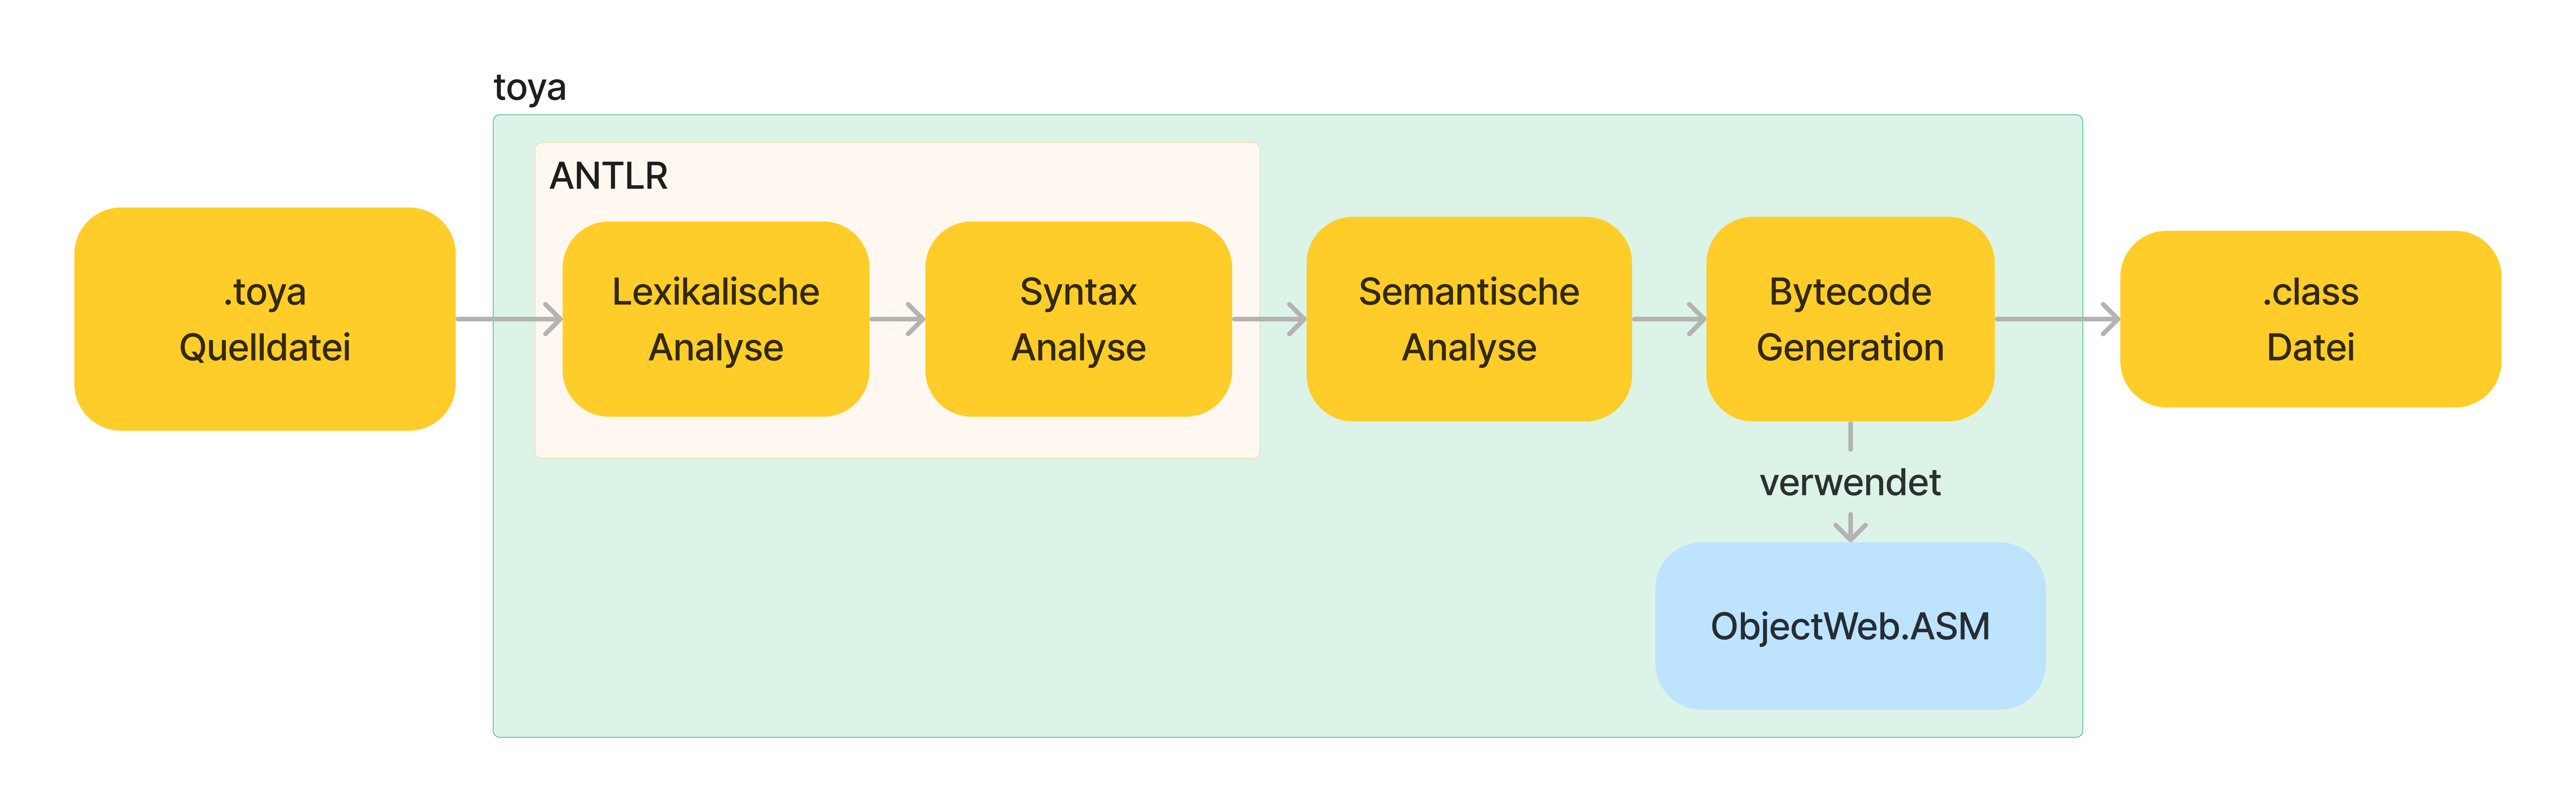
\includegraphics[width=\textwidth]{Compiler.Architecture}
    \label{fig:compiler-architecture}
\end{figure}

\section{Frontend}

Im Frontend erfolgt die lexikalische, syntaktische und teilweise die semantische Analyse. Die lexikalische Analyse zerlegt anhand der bereitgestellten Grammatik den Quellcode in \token. Anhand dieser \token erstellt die syntaktische Analyse den Syntaxbaum, welcher als Basis für den abstrakten Syntaxbaum dient.

\subsection{Grammatik}

Als Ausgangspunkt des Frontends dient die Grammatik, anhand welcher ANTLR die lexikalische und syntaktische Analyse implementiert. Diese Grammatik definiert die Compiler-Bauer:in in einer \texttt{g4}-Datei. Leerzeichen haben keine semantische Relevanz, weshalb \toya diese in der syntaktischen Analyse überspringt. Als \token definiert \toya folgende Zeichen:

\begin{itemize}
    \item Die Schlüsselwörter \texttt{match}, \texttt{for}, \texttt{for}, \texttt{if}, \texttt{else}, \texttt{var}, \texttt{true}, \texttt{false} und \texttt{null}
    \item Die Infix-Operatoren \texttt{>}, \texttt{>=}, \texttt{<}, \texttt{<=}, \texttt{==}, \texttt{!=}, \texttt{\&\&}, \texttt{||} und der Präfix-Operator \texttt{!}
    \item Die arithmetischen Operatoren \texttt{+}, \texttt{-}, \texttt{*} und \texttt{/}
\end{itemize}

Beim Versuch, ein Schlüsselwort als Variablenname zu Verwenden tritt ein Ausnahmezustand \texttt{VariableNameIsKeywordException} ein. 

\begin{ToyaCode}[numbers=none, caption={Befehl zur Erzeugung der Visitor-Klassen für \toya}]
antlr4 -o C:\home\Lukas\projects\toya\src\main\java\gen \
    -package gen \
    -Dlanguage=Java \
    -visitor \
    -no-listener \
    -lib C:/home/Lukas/projects/toya/src/main/resources \
    C:/home/Lukas/projects/toya/src/main/resources/toya.g4
\end{ToyaCode}

\subsection{Abarbeitung des Syntaxbaum}

Wie bereits im Kapitel Generierung des Syntaxbaum\ref{cha:antlr} erläutert, bietet ANTLR die Entwurfsmuster \visitor und \listener an, um den Syntaxbaum zu traversieren. \Toya verwendet das \visitor-Muster aufgrund des Umfangs des zu traversierenden Syntaxbaums. Das Resultat des \visitors ist ein AST mit dem Wurzelelement \texttt{Compilation}. Diese Klasse speichert die Funktionssignaturen, globale Variablen und ein globales \scope, welches sich über das ganze Programm erstreckt. Alle weiteren \texttt{Scopes} nehmen dieses globale \scope als Grundlage. 

Die wichtigste Methode des \visitor, welche die Abarbeitung des Syntaxbaums überhaupt ermöglicht ist die \texttt{accept()} Methode. Diese Methode benötigt als Parameter einen \visitor vom generischen Typ \texttt{ParseTreeVisitor}. \Toya implementiert folgende \visitor:

\begin{itemize}
    \item CompilationVisitor
    \item StatementVisitor
    \item BranchVisitor
    \item CompositeVisitor
    \item ExpressionVisitor
    \item FunctionSignatureVisitor
    \item FunctionVisitor
\end{itemize}

Zum traversieren des Syntaxbaums generiert ANTLR für jede Regel in der Grammatik-Definition eine Methode im Format \texttt{visit<RuleName>(ctx: toyaParser.<RuleName>Context)}. Jede dieser Methoden liefert einen Wert zurück, der dem generischen Typ des \texttt{toyaBaseVisitor} entspricht.

\begin{KotlinCode}[numbers=none, caption={\visitor-Funktion zum Erstellen eines \texttt{VariableDeclarationStatement}}]
class StatementVisitor(val scope: Scope) : toyaBaseVisitor<Statement>() {
    override fun visitVariableDeclaration(ctx: toyaParser.VariableDeclarationContext): Statement {
        val varName = ctx.name().text
        if(varName.isReservedKeyword()) throw VariableNameIsKeywordException(varName)
        val expression = ctx.expression().accept(ExpressionVisitor(scope))
        scope.addLocalVariable(LocalVariable(varName, expression.type))
        return VariableDeclarationStatement(varName, expression)
    }
    // Rest of class
}
\end{KotlinCode}

Befinden sich Syntaxfehler im Quelltext, bietet ANTLR die Basisklasse \texttt{BaseErrorListener} um der Benutzer:in relevante Informationen anzuzeigen. \Toya zeigt mithilfe dieser Klasse an, welche Anweisung in welcher Zeile und welches Zeichen syntaktische syntaktische Analyse verhindert.

\begin{KotlinCode}[numbers=none, caption={Erstellen des \visitor}]
class Parser {
    fun getCompilation(files: List<File>): Compilation {
        return files.use {path ->
            val charStream = CharStreams.fromPath(path)
            val lexer = toyaLexer(charStream)
            val tokenStream = CommonTokenStream(lexer)
            val parser = toyaParser(tokenStream)

            val errorListener = ToyaTreeWalkErrorListener()
            parser.addErrorListener(errorListener)

            val compilationVisitor = CompilationVisitor()
            parser.compilation().accept(compilationVisitor)
        }
    }
}
\end{KotlinCode}

\subsection{Typ-System}

Die Basis für das Typ-System in \toya ist die \texttt{Type}-Schnittstelle und die davon abgeleitete Enum-Klasse \texttt{BasicType}, welche alle in \toya verfügbaren Typen zur Verfügung stellt. \Toya erlaubt keine explizite Definition des Typs einer Variable, weshalb der Typ immer vom Wert der Variable abzuleiten ist. Hierbei kommt der \texttt{TypeResolver} zum Einsatz. Anhand von regulären Ausdrücken ermittelt dieser den Typ des Wert-Literals.

\begin{KotlinCode}[numbers=none, caption={Methode zur Ermittlung des Typs bei Wert-Literalen}, label={lst:getFromValue}]
fun getFromValue(value: String?): Type {
    if (value.isNullOrEmpty()) return BasicType.VOID
    if (isBoolean(value)) return BasicType.BOOLEAN
    if (isDouble(value)) return BasicType.DOUBLE
    if (isInt(value)) return BasicType.INT
    if (isString(value)) return BasicType.STRING
    throw UnableToInferTypeException(value)
}
\end{KotlinCode}

\texttt{TypeResolver} bietet außerdem Hilfsmethoden zur individuellen Behandlung von Typen. Diese Methoden kommen zum Einsatz bei der Generierung der Bytecode Anweisungen, da jeder Typ unterschiedliche Anweisungen verlangt. So ist zum Laden von Zeichenketten zum Beispiel \texttt{ALOAD} nötig, wohingegen für Ganzzahlen \texttt{ILOAD} zu verwenden ist.

\begin{KotlinCode}[numbers=none, caption={Hilfsmethode zur Behandlung der Nicht-Feld Typen}]
fun <T> Type.handleTypeGroups(
    i: () -> T,
    d: () -> T,
    a: () -> T,
    z: () -> T
): T {
    return when (this) {
        BasicType.INT -> i()
        BasicType.DOUBLE -> d()
        BasicType.STRING -> a()
        BasicType.BOOLEAN -> z()
        else -> throw NotImplementedError("handling for type '\${this.typeName}' not implemented")
    }
}
\end{KotlinCode}

Da nun die jeder Ausdruck Typinformationen besitzt, ermöglicht das die semantische Analyse von Ausdrücken. Die Funktion \texttt{checkTypeMatch()} überprüft, ob beide Operanden vom selben Typ sind. Wenn nicht, wechselt das Programm in einen Ausnahmezustand.

\begin{KotlinCode}[numbers=none, caption={Methode zur Überprüfung, dass Operanden übereinstimmende Typen haben}]
fun Type.checkTypeMatch(rhs: Type) {
    if (this != rhs) throw BinaryOperationTypeMismatchException(this, rhs)
}    
\end{KotlinCode}

\subsection{Standardfunktionen}

\Toya bietet keine Standardbibliothek, jedoch aber die Möglichkeit Standardfunktionen zu implementieren. Standardfunktionen sind kein Bestandteil der lexikalischen Analyse. Stattdessen überprüft die Funktion \texttt{visitFunctionCall} des \texttt{ExpressionVisitors} mithilfe der Funktion \texttt{isStandardFunction()}, ob es sich um eine Standardfunktion handelt. Ist dies der Fall, erzeugt der \visitor kein Objekt vom Typ \texttt{FunctionCall}, sondern ein Objekt, welches von \texttt{StandardFunction} erbt. Im Fall von \texttt{print()} ist das zum Beispiel \texttt{PrintFunction}.

Standardmäßig bietet \toya die Standardfunktion \texttt{print()} an, welche einen Aufruf der Java Funktion \texttt{System.out.println()} durchführt. Die Architektur des \toya-Compilers ist darauf ausgelegt, weitere Standardfunktionen hinzufügen zu können. Besteht dieser Wunsch, sind an folgenden Stellen von Entwicklerseite her Veränderungen vorzunehmen:

\begin{itemize}
    \item Im \texttt{when} innerhalb der \texttt{ExpressionVisitor.visitFunctionCall()} Funktion muss ein Fall für die zu implementierenden Funktion hinzugefügt werden.
    \item Innerhalb der \texttt{StandardFunctions.kt} Datei: In der \texttt{standardFunctions} Liste ist eine FunktionsSignatur der neuen Standardfunktion hinzuzufügen und eine Klasse, welche von \texttt{StandardFunction} und \texttt{Expression} erbt, zu definieren.
    \item In der \texttt{StandardFunctionGenerator} Klasse ist der zu generierende Bytecode zu definieren.
\end{itemize}

\section{Abstrakter Syntaxbaum (AST)}

Die explizite Umwandlung auf einen abstrakten Syntaxbaum ist theoretisch nicht immer nötig. \toya verwendet aber ANTLR und der daraus resultierende Syntaxbaum enthält teilweise zu viele Informationen. Teilweise fehlen auch notwendige Informationen, wie zum Beispiel die über den Typ eines Ausdrucks. Daher macht es Sinn, diesen Syntaxbaum auf einen abstrakten Syntaxbaum (AST) umzubauen. Der großteil des AST behandelt die Einteilung von Ausdrücken und Anweisungen in ein granulareres Klassen-Schema. Die Einteilung in zum Beispiel \texttt{LessEqualExpression} und \texttt{ForStatement} anstatt die bloße Gliederung in \texttt{Expression} und \texttt{Statement} ermöglicht eine gut skalierbare und verständliche Lösung für die Bytecode-Generierung. 

\begin{figure}
    \caption{AST-Architektur für Ausdrücke und Anweisungen}
    \centering
    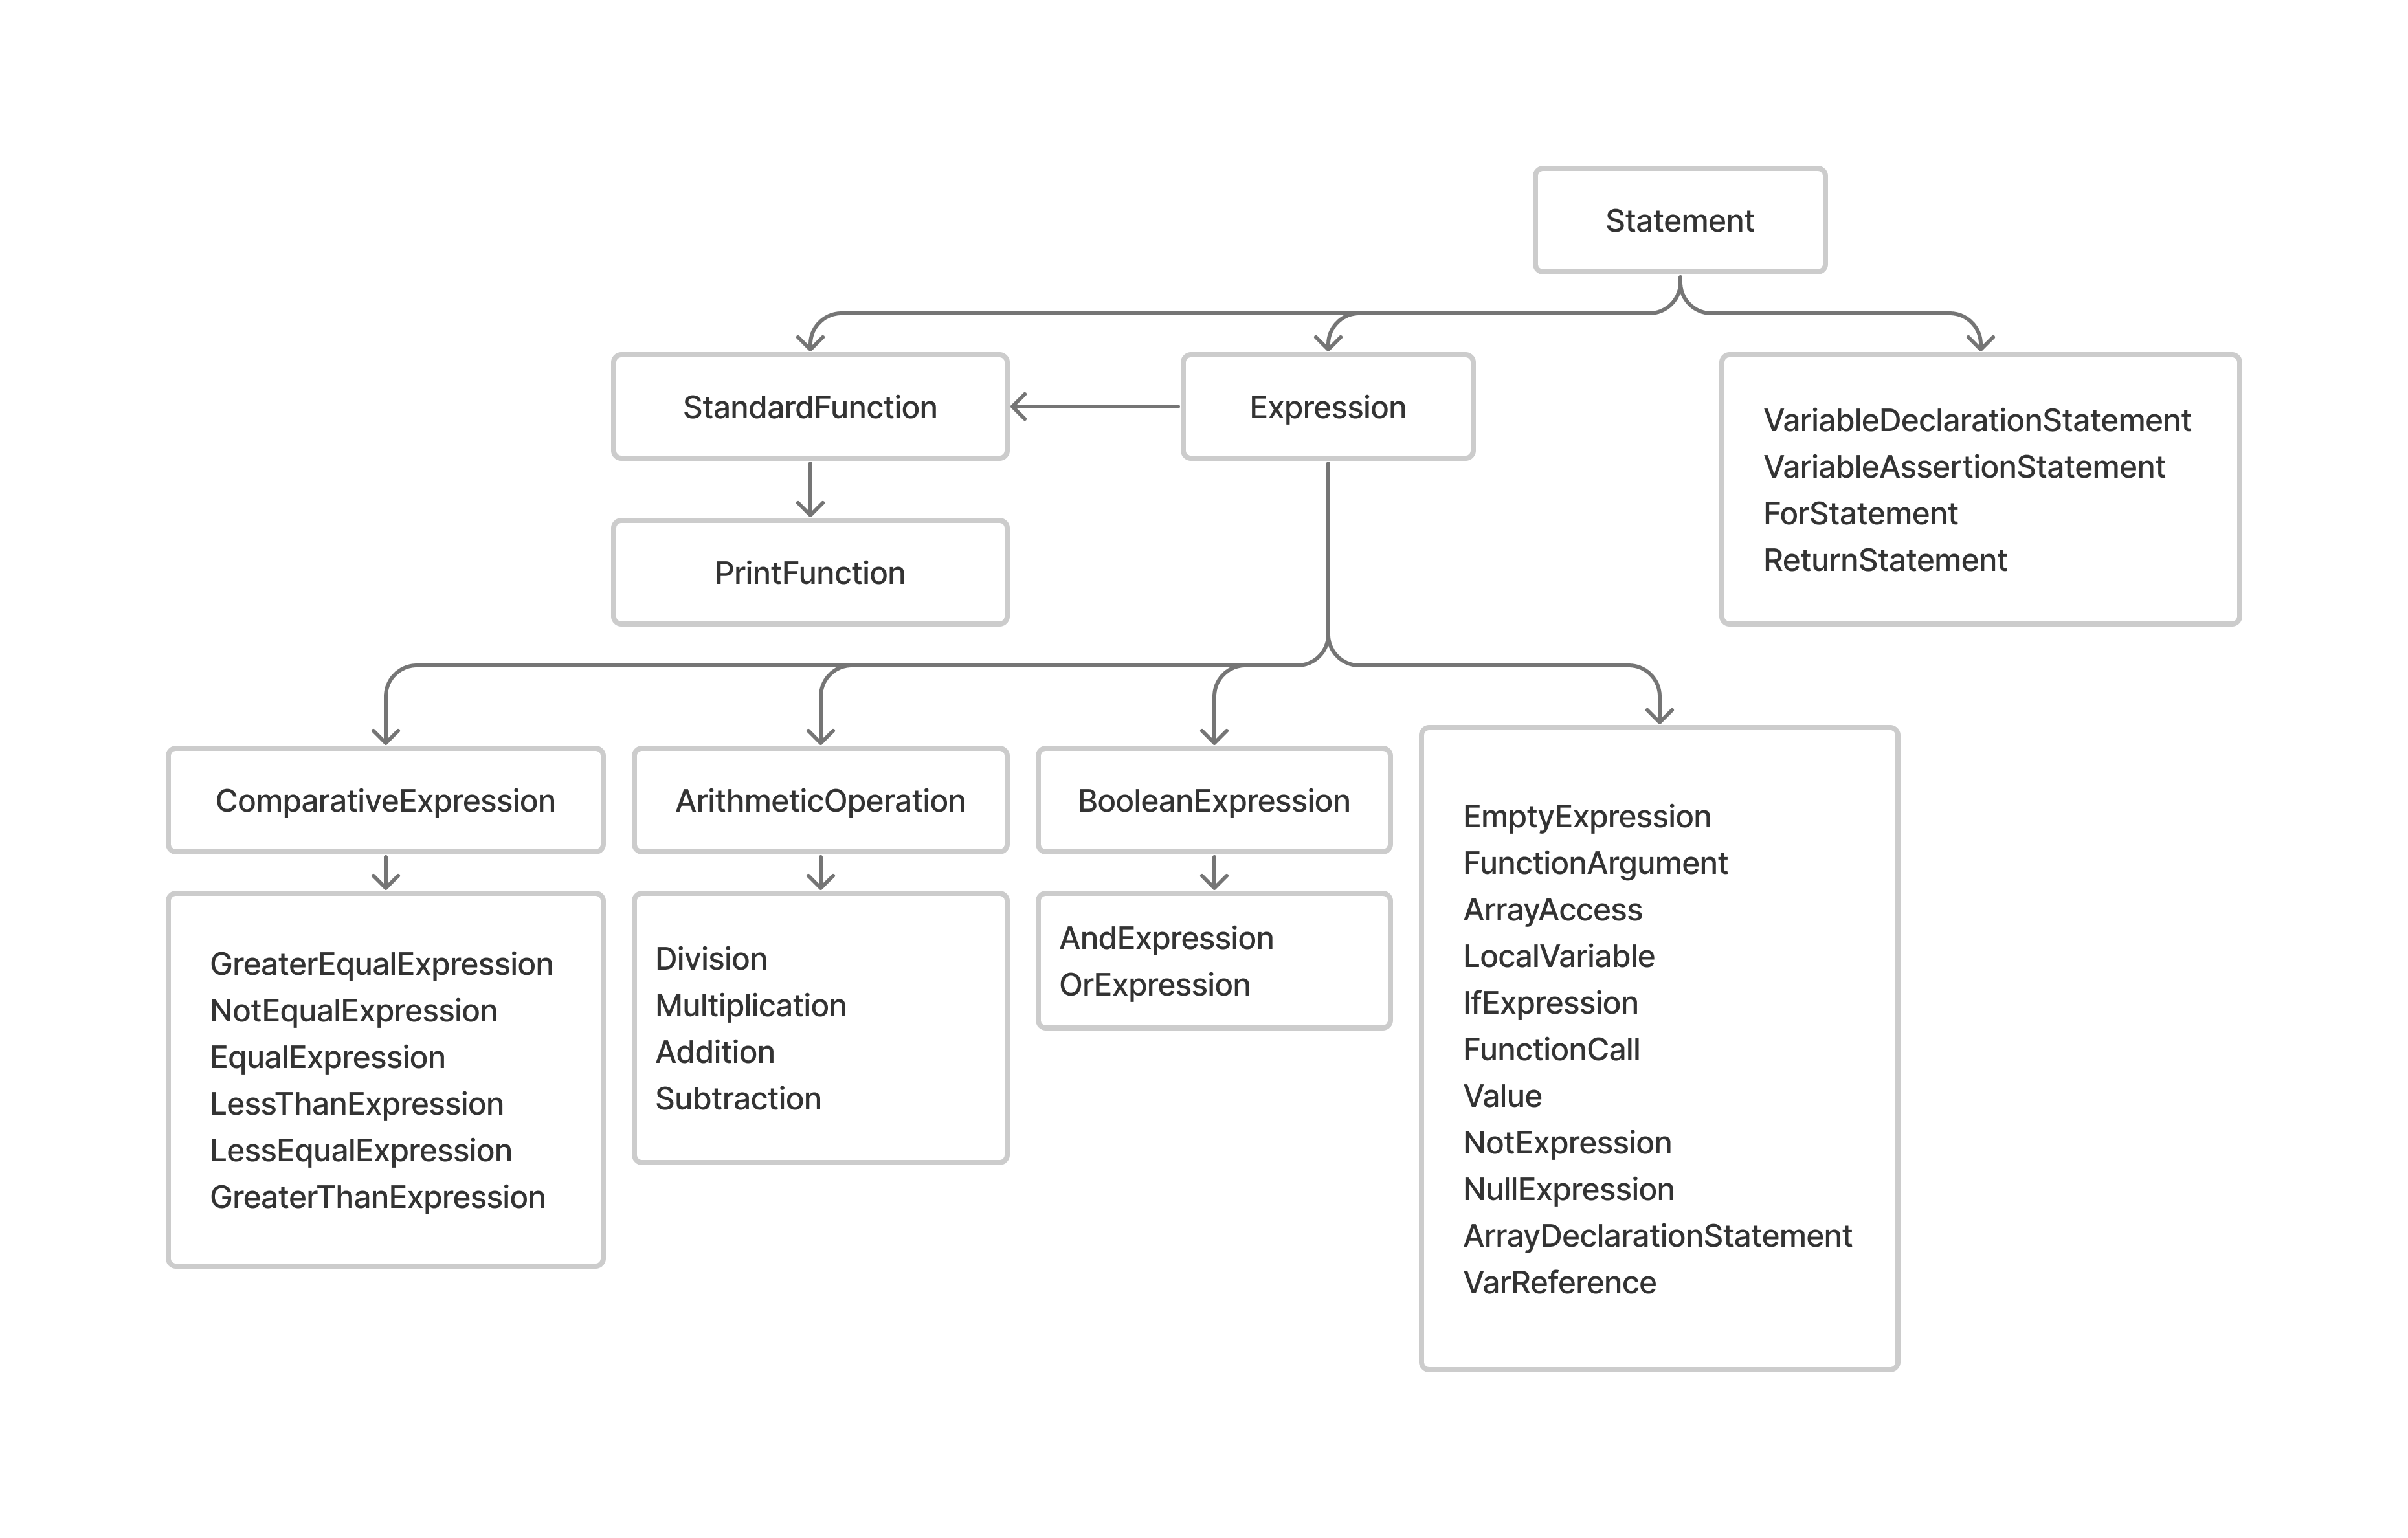
\includegraphics[width=\textwidth]{AST.Diagram}
    \label{fig:ast-architecture}
\end{figure}

Kotlin bietet zur kompakten Erstellung von Datenobjekten sogenannte \textit{data classes} an. \texttt{data class} Objekte erzeugen für Mitglieder des primären Konstruktor folgende Funktionen:

\begin{itemize}
    \item \texttt{equals()} und \texttt{hashCode()}.
    \item \texttt{toString()} im Format \texttt{Addition(left=42, right=31)}.
    \item \texttt{componentN()}, die bei der Destrukturierung von Objekten verwendet werden. Hierbei ist die angegebene Reihenfolge relevant.
    \item \texttt{copy()} zum durchführen einer tiefen Kopie des Objekte.
\end{itemize}

\Toya verwendet \textit{data classes} für fast alle Klassen des AST. Ausgenommen sind Basisklassen, von denenen andere Klassen ableiten, da die Vererbung von \textit{data classes} zu Problemen mit dem Verhalten von \textit{equals()} zum Beispiel führt. Java bietet seit Version 14 \texttt{record} als Äquivalent zu diesem Konzept an. Jedoch fehlen bei \texttt{record} die \texttt{copmonentN()} und \texttt{copy()} Funktionen.

Die \texttt{Scope} Klasse ist eine zentrale Komponente in der Verwaltung des AST und wird unter anderem für die semantische Analyse benötigt. Sie speichert die lokalen Variablen für einen gegebenen Block und die Methodensignaturen eines \toya Programms. Bei Operationen, deren Operanden lokale Variablen sind, überprüft \toya mithilfe \texttt{Scope}, ob diese Variablen im momentanten Kontext zur Verfügung stehen.

Im Zuge der Bytecode-Generierung ermittelt \toya mithilfe \scope den Index einer lokalen Variable. Hierbei reicht es nicht aus, den Index der Variable in der Liste \texttt{localVariables} zu ermitteln. Variablen vom Typ \texttt{Double} und \texttt{Long} benötigen zwei Plätze im \textit{Run-Time Constant Pool}, da deren Indizes 16 Bit, anstatt der üblichen acht Bit einnehmen. Da \toya den Typ Double implementiert, ist diese Eigenschaft zu berücksichtigen. Diese Berechnung erfolgt durch eine Reduktions-Operation in der Funktion \texttt{getLocalVariableIndex}. Diese Reduktions-Operation summiert alle Indizes bis inklusive dem Index der gesuchten Variable auf und addiert pro Index eins, beziehungsweise zwei, wenn die Variable vom Typ Double ist, mit dem Akkumulator auf.

\begin{KotlinCode}[numbers=none, caption={Ermittlung des Index einer Variable in einem \texttt{Scope}}]
fun getLocalVariableIndex(varName: String) : Int {
    // hotfix for handling 2-wide index types (double, long, etc)
    return localVariables
        .subList(0, localVariables.indexOf(getLocalVariable(varName)))
        .fold(0) { acc, next ->
            acc + if (next.type == BasicType.DOUBLE) 2 else 1
        }
}
\end{KotlinCode}

\texttt{Scope} verwaltet nicht nur Variablen, sondern auch Funktionssignaturen. Beim Aufruf einer Funktion, überprüft \scope, ob diese Funktion auch definiert ist. Wenn nicht, tritt der Ausnahmezustand \texttt{MethodSignatureNotFoundException} ein. Während das Überladen von Funktionen erlaubt ist, können keine Funktionen mit identischer Signatur existieren, da diese in einem \texttt{Set} gespeichert sind.

\section{Backend}

\subsection{ObjectWeb ASM}

ObjectWeb ASM ist eine Bibliothek zum Lesen, Bearbeiten und Erzeugen von Bytecode für die JVM. Sie bietet eine Schnittstelle, um Funktionen, Klassen und einzelne Anweisungen zu erzeugen. \toya verwendet ASM zum Erzeugen einer Klasse und Funktionen anhand des AST. Neben der Bytecode-Generierung erfolgt im Backend der Teil der semantischen Analyse für welchen Informationen des AST notwendig sind.

Da \toya keine Definition von Klassen erlaubt, reicht es aus, eine statische Klasse, unabhängig von Quelltext zu generieren. Version dieser Klasse ist 52, was Java 8 entspricht. Einen höhere Version ist nicht nötig, da alle Bestandteile von \toya sehr primitiv sind.

Klassen erstellt ASM mithilfe des \texttt{ClassWriter}. Der Konstruktor dieser Klasse hat einen Parameter \texttt{flags}. Im Falle von \toya ist dies \texttt{COMPUTE\_FRAMES + COMPUTE\_MAXS}. \texttt{COMPUTE\_MAXS} und \texttt{COMPUTE\_FRAMES} ermöglicht die automatische Berechnung der maximal erlaubten Anzahl an lokalen Variablen, die maximale Größe des Stacks und die Berechnung aller \textit{Stack Map Frames}.

\begin{KotlinCode}[numbers=none, caption={ASM Code zum Erstellen der Klasse, welche ein \toya Programm definiert.}]
val classWriter: ClassWriter = ClassWriter(
    ClassWriter.COMPUTE_FRAMES + ClassWriter.COMPUTE_MAXS
)
classWriter.visit(
    CLASS_VERSION,
    Opcodes.ACC_PUBLIC,
    className,
    null,
    "java/lang/Object",
    null
)
\end{KotlinCode}

Im Backend kommen Summen Typen in Form von \textit{sealed classes} zum Einsatz. \textit{sealed classes} in Kotlin besitzen die besondere Eigenschaft, dass alle Kindklassen zur Übersetzungszeit vollständig bekannt sind. Dies ermöglicht zum Beispiel die Verwendung von erschöpfenden \texttt{when}-Ausdrücken in Kombination mit Polymorphismus. Kindklassen einer \textit{sealed class} sind alle im selben Modul zu definieren. Neben Klassen können auch Schnittstellen als \texttt{sealed} markiert werden.

\begin{KotlinCode}[numbers=none, caption={Die \texttt{generate()} Funktion von \texttt{StatementGenerator}, welche \textit{sealed classes} nutzt.}]
fun generate(statement: Statement, scope: Scope) {
    when (statement) {
        is VariableDeclarationStatement -> generate(statement, scope)
        is ArrayDeclarationStatement -> generate(statement, scope)
        is VariableAssertionStatement -> generate(statement, scope)
        is Expression -> expressionGenerator.generate(statement, scope)
        is ReturnStatement -> generate(statement, scope)
        is ForStatement -> generate(statement)
    }
}
\end{KotlinCode}

Die JVM ist eine Stack-basierte virtuelle Maschine. Das bedeutet, dass ein Operanden-Stack existiert, auf welchen alle Werte, die die Bytecode Anweisungen benötigen, liegen.

\begin{KotlinCode}[numbers=none, caption={\texttt{generate()} Funktion, welche Wert-Literale erzeugt.}]
private fun generate(value: Value) {
    val type = value.type
    val stringValue = value.value

    type.handleTypeGroups(
        i = {
            val intValue = stringValue.toInt()
            methodVisitor.visitLdcInsn(intValue)
        },
        d = {
            val doubleValue = stringValue.toDouble()
            methodVisitor.visitLdcInsn(doubleValue)
        },
        a = { methodVisitor.visitLdcInsn(stringValue.trim('"')) },
        z = {
            val opcode = if (stringValue == "true") Opcodes.ICONST_1 else Opcodes.ICONST_0
            methodVisitor.visitInsn(opcode)
        }
    )
}
\end{KotlinCode}